The purpose of this chapter is to introduce the background and main concepts required to describe and compare self-reconfiguring robotic systems.
The beginning of this chapter includes a section of related work comparing similar projects and experiments.
Following, this chapter reviews the state-of-the-art of self-assembly mechanisms.
This includes the assembly architecture, protocol and different hardware mechanisms for real world application.
This chapter also reviews any additional theory that is needed for the implementation and analysis of this experiment such as machine learning and artificial neural networks.

\section{Related work}
Self-assembly in robotics is a relatively new field of research, however there are still some papers which attempts to discuss and compare the different mechanisms in a self-assembly system. 
\cite{murata_self-reconfigurable_2007} mainly covers the potential of reconfigurable systems, as well as the challenges of self-reconfigurable robotics. 
Though this article does not conduct any experiment, it does touch upon some of the same issues that this report is trying to outline.

\cite{yim_modular_2002} is an article released in 2002 that tries to explain how modular robots can self-reconfigure to solve different tasks. 
In particular, this article looks at \emph{PolyBot} and how it is able to reconfigure into different shapes. 
\cite{yim_modular_2002} also covers some of the benefits in general of having a self-reconfigurable system, as well as challenges that are still being explored.

\cite{yim_modular_2007} is the more complete and detailed of the articles presented here. 
In addition to the general benefits and challenges of modular self-reconfigurable robot system, it also looks at the different architectures the system can take, application areas and history of the field.
The article also includes an extensive list containing many self-reconfigurable modular systems and the type of architecture they have.

These papers outline what a modular self-reconfigurable system is and what the benefits and challenges of these systems are.
However, there are no direct comparison between the mechanisms themselves.
\cite{yim_modular_2007} introduces many different systems that work quite differently, but there is no conclusion based on if  these systems promote self-assembly or not.

\section{Complex systems}
\label{sec:complex_systems}
What separates complex systems from what we determine "simple systems" is that the behaviour of the system cannot be understood by simply looking at individual parts of the system.
The way the parts act together and how they are connected is what gives rise to complex behaviour.
This concept bring us to emergent behaviour.
Emergent behaviour is a process where the system takes on certain patterns, regularities or form larger entities through the interconnections and interactions among simple parts that by themselves to not portray such properties.
Further, this report will look at an emergent behaviour known as self-assembly.  

In nature one can find many examples of complex systems displaying self-organizing behaviour.
The collectives range from just a few individuals to millions.
Some examples are flocking behaviour in birds, fish schooling, and the complex societies seen among social insects(Figure \ref{fig:collective-behaviour}). 

\begin{figure}[H]
	\centering
	\begin{subfigure}[b]{0.31\textwidth}
		\label{fig:flocking}
		\centering
		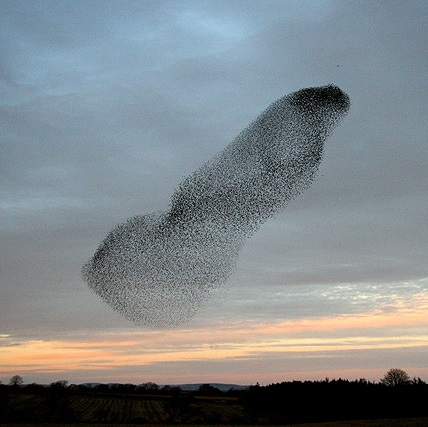
\includegraphics[height=\linewidth]{chapters/res/flocking_edit.jpg}
		\caption{Flocking\cite{baxter_flocking.jpg_2008}}
	\end{subfigure}
	\begin{subfigure}[b]{0.31\textwidth}
		\label{fig:scholing}
		\centering
		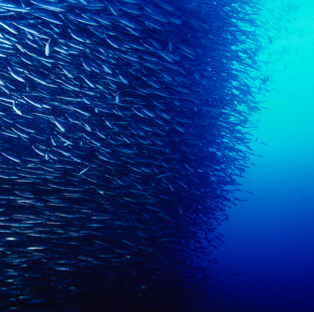
\includegraphics[height=\linewidth]{chapters/res/schooling_edit.png}
		\caption{Schooling\cite{polyglottus_mockingbird-tales-readings--animal-behavior-5.1.pdf_2011}}
	\end{subfigure}
	\begin{subfigure}[b]{0.31\textwidth}
		\label{fig:social-insects}
		\centering
		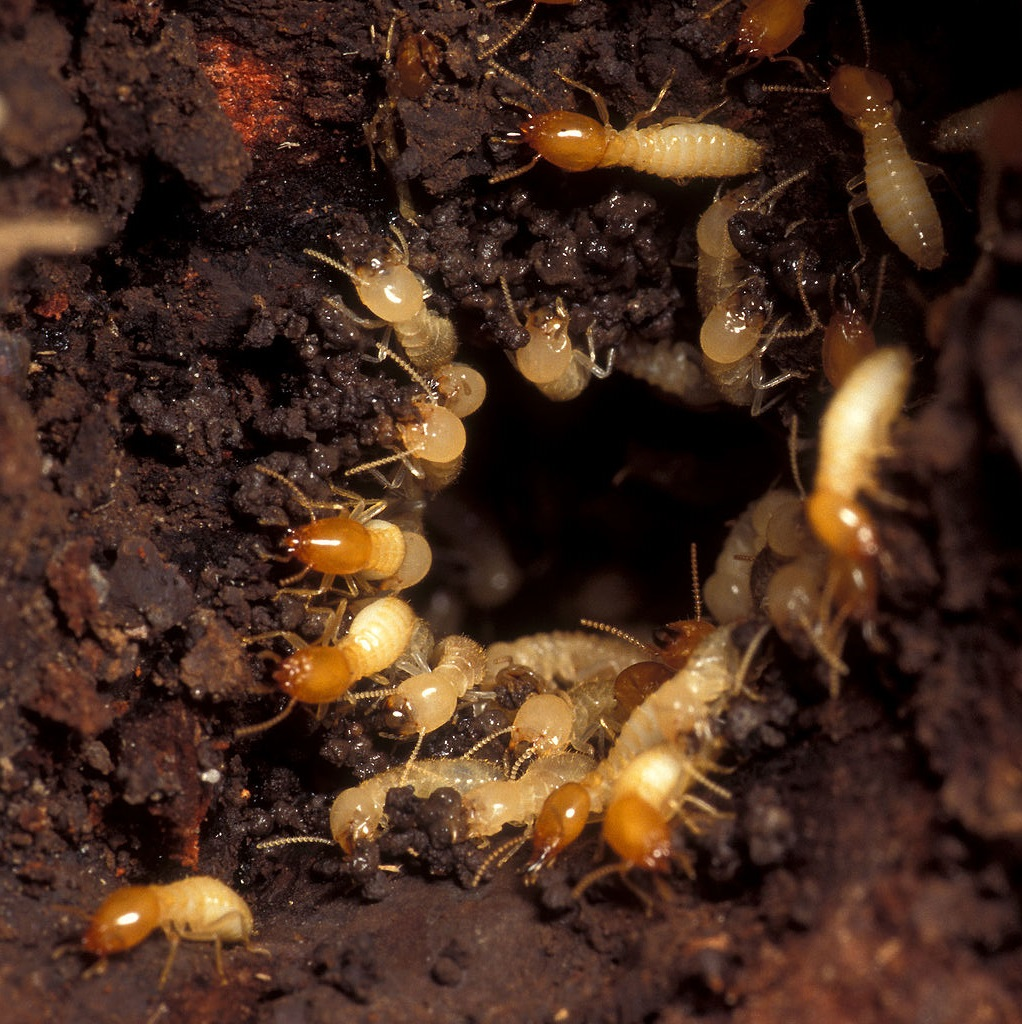
\includegraphics[height=\linewidth]{chapters/res/Termites_rush_to_damaged_portion_of_mound_edit.jpg}
		\caption{Termites\cite{bauer_termites_rush_to_damaged_portion_of_mound.jpg_2007}}
	\end{subfigure}
	\caption{Examples of self-organizing behaviour in nature.}
	\label{fig:collective-behaviour}
\end{figure}

Social insects such as termites build large structures featuring complex architectures.
These examples show how a collective of simple agents, without a central controller can accomplish tasks each individual would be unable to perform themselves. 
Together, the actions of these agents form a collective behaviour that can be considered intelligent.  

These biological systems display massively parallel, decentralized computation.
This stands in contrast to conventional computer systems with a central processing unit executing instructions serially.
Research into self-assembling robot systems therefore take inspiration from biology, using methods such as evolutionary algorithms simulating Darwinian evolution, and artificial neural networks inspired by the way brains process data.




\section{Self-assembly architectures}
\label{sec:sfArchitecture}
Self reconfiguring robots can assemble into many different shapes, and there are many ways to do so.
We define these properties as the self-assembly architecture.
Each architecture presents different challenges and benefits.
The architectures can in broad terms be categorized either as non-mobile- or mobile-architectures.
The non-mobile architectures are characterized by the topologies of the structures they form, while mobile architectures are characterized by having more mobile robots with a higher degree of freedom.
This section will describe and define some of the common assembly architectures used in previous projects.
\subsection{Non-mobile Architecture}
Typically these robots have little mobility themselves, but can form complex structures capable of a wide range of behavior.
One of the long term visions for these kinds of robots is called "bucket of stuff"\cite{yim_modular_2007}.
The idea is to have a collection of different robot modules which can be assembled on demand to solve different tasks.
One way to classify non-mobile robots is based on their configuration topology.
The main classes for configuration topologies are chain and lattice configurations.
\subsubsection{Chain topology}
The chain topology is a configuration where each robot is connected in a serial architecture.
The robots can form many different shapes to represent creatures such as snakes, spiders or other configurations needed to complete its task.
One of the challenges with this topology is coordinating movement and decisions as information has to be propagated serially.
Examples of chain architecture based robots are Molecubes\cite{zykov_molecubes:_2007}, Yamor\cite{mockel_yamor_2006}, and Conro\cite{castano_conro:_2000}.
Yamor is depicted in figure \ref{fig:yamor}.
\begin{figure}[H]	
	\centering
	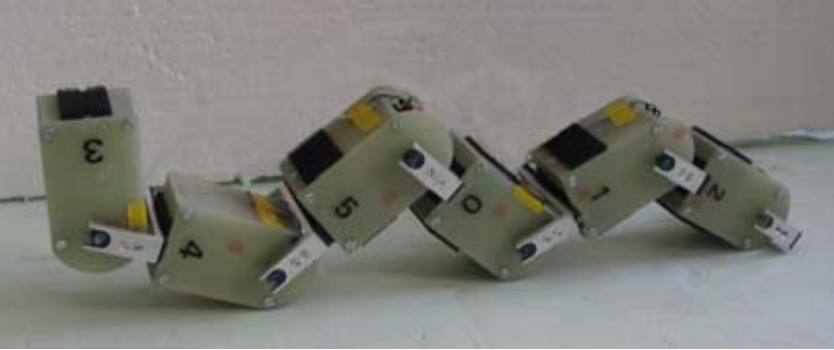
\includegraphics[scale=0.5]{chapters/res/Yamor.PNG}
	\caption{Yamor robots configured as a snake\cite{mockel_yamor_2006}.}
	\label{fig:yamor}
\end{figure}

\subsubsection{Lattice topology}
The Lattice architecture is a configuration where robots are arranged in a grid/lattice topology.
The robots can then execute motion and control in parallel which provides a simpler configuration in comparison to the chain architecture. 
Examples of lattice architecture would be a cubic or hexagonal grid.
Due to its simplicity, a lattice architecture is easier to scale. 
There have been more research groups working on this class of architecture due to its easier implementation \cite{yim_modular_2002}.

Symmetry is a desirable property for robots that employ the lattice architecture because this makes reconfiguration into new positions in the grid easier.
To maintain the symmetry property in 3D space, each robot needs more connection points and actuators than in 2D space\cite{murata_self-reconfigurable_2007}.
This complicates the design of the robots. 
Thus, building these robots with a high enough power/weight ratio is difficult.
Examples of lattice architecture based robots which is able to perform self-reconfiguration are ATRON\cite{brandt_atron_2007}, Miche\cite{gilpin_miche:_2008}, and Catoms\cite{kirby_catoms:_2005}.
Atron is depicted in figure \ref{fig:atron}.

\begin{figure}[H]
	\centering
	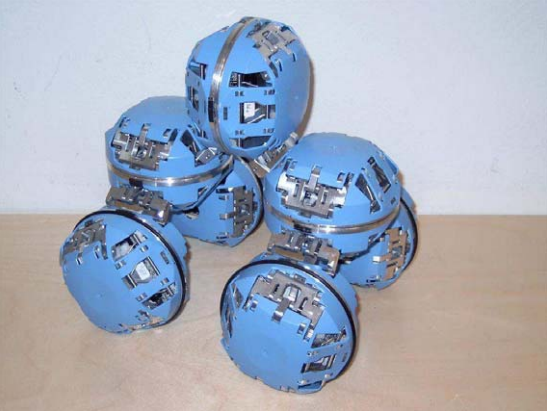
\includegraphics[scale=0.5]{chapters/res/Atron.png}
	\caption{Atron assembled into a four wheeled car \cite{brandt_atron_2007}.}
	\label{fig:atron}
\end{figure}

\subsection{Mobile architecture}
Mobile architectures are characterized by having autonomous robots which can self-assemble and reconfigure themselves.
Each robot can operate independently or form larger structures when needed, by hooking up with other units.
The structures formed may have different topologies and can coordinate their movements to form a larger virtual network\cite{yim_modular_2007}.
One example of a mobile architecture is presented in \cite{gross_object_2006}.
In the experiment depicted in figure \ref{fig:swarmbot-object-transport}, a group of robots are programmed  to move an object which requires cooperation by being to heavy for a single robot to move.

\begin{figure}[H]
	\centering
	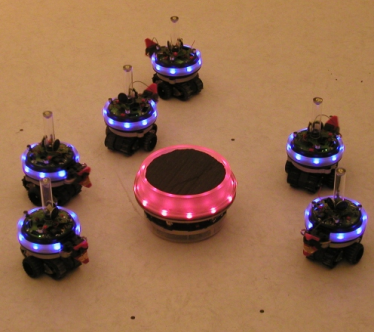
\includegraphics{chapters/res/MobileObjectTransport.png}
	\caption{A group of swarmbots(blue) preparing to transport an object(red)\cite{gro_autonomous_2006}.}
	\label{fig:swarmbot-object-transport}
\end{figure}
Since each robot in the architecture is autonomous one challenge is making the individual robots cooperate.
This is especially difficult in cases where the optimal solution to a task involves cooperation, but the robots are able to complete the task individually.
This challenge is demonstrated in \cite{trianni_evolving_2004} where the researchers were able to promote self-assembly to solve the task, but the self-assembly was only present in 2 out of 10 trials.

The high degree of mobility in each robot allows them to form a wide variety of topologies to solve tasks, but this also makes reconfiguration more difficult for large robot swarms.
Because of this difficulty there has been less research into mobile architectures.

Experiments conducted demonstrates robots solving simple tasks such as object transport\cite{gro_autonomous_2006}, phototaxis\cite{trianni_evolving_2004}, and energy collection\cite{montanier_adaptive_2014}\cite{weel_emergence_2012}.
These experiments demonstrate that mobile robots are capable of solving tasks through self-assembly.
But the tasks presented are trivial problems and do not reflect the complexity of real world problems.
Before solving real world problems, future research need to demonstrate a greater amount of robots cooperating.
Additionally, robots that have the ability to take different roles when solving problems as well as cooperating when solving multiple problems presented by the environment.

\section{Hardware mechanisms}
\label{sec:hardware}
Several robot systems that are capable of self-assembly have been developed over the years\cite{gross_self-assembly_2008}\cite{wei_sambot:_2011}\cite{brandt_atron_2007}.
Even though some vary greatly in implementation, all these robots have some sort of hardware which makes it possible to perform self-assembly.
The hardware available in each robot is influenced by the desired assembly architecture.
However, some common properties can be identified.  

\section*{Prerequisites for self-assembly}
The robots must have some form of \emph{movement} to reach each other.
This movement can be provided by the hardware available or from external sources.
Similar to movement, the robots require a \emph{docking mechanism} to physically connect to other robots in order to self-assemble.

The requirements described can be considered as minimum requirements for self-assembly, but for more advanced behaviour, the robots need additional hardware utilities.
If the robots are to be self-assembled without human intervention, they need a \emph{discovery mechanism} to detect the presence of each other.
To coordinate behaviour, the robots also need a \emph{communication mechanism} capable of receiving and sending information.
These requirements are very general and can be achieved in a wide variety of ways. Table \ref{tab:hardware-mechanisms} describes some methods to complete the discovery and communication requirements.

\begin{table}[H]
	\centering
	
	\begin{tabular}{ | l | l | l |p{5cm} |}
		\hline
		& Chain 						& Lattice \\ \hline
		Discovery 		& IR\cite{castano_conro:_2000}  & IR\cite{gilpin_miche:_2008} \\ \hline
		Communication 	& 1-wire bus\cite{zykov_molecubes:_2007}, IR\cite{castano_conro:_2000}, Bluetooth{\cite{mockel_yamor_2006}} & IR\cite{brandt_atron_2007},\cite{gilpin_miche:_2008}  \\\hline
	\end{tabular}
	\caption{Various hardware solutions to discovery and communication.}
	\label{tab:hardware-mechanisms}
\end{table}


It is possible to simplify or ignore some of these requirements, but self-assembly is impossible without the docking mechanism.
This means that the choice of docking mechanism can be a deciding factor in the performance of a self-assembling robot. 


\subsection{Docking mechanisms}
\label{sec:mechanisms}
The docking mechanism is an essential component in self-assembly, and has been solved in various ways in previous studies.
For experiments with self-assembly in simulation, the mechanisms are often simplified since the focus of the experiments usually is the self-assembly behaviour.
Therefore, it can be difficult to replicate the results on real hardware.
The real world introduces noise, and the mechanisms designed must be able to cope with that imperfection.
This is especially true in the context of machine learning as the resulting controllers are rarely optimal.
The desired self-assembly architecture also plays a role in designing a docking mechanism.

\subsubsection*{Male-female connector}
This form of connection mechanism is used by the ATRON\cite{brandt_atron_2007} robots.
The male modules are shaped like three hooks that can lock onto female connector bars.
Each robot has eight connector modules, and are arranged such that every second connector is male and every second is female.
This allows each robot to connect to a maximum of eight other robots.
A disadvantage with this type of mechanism is that the robots have to match the male to the female connectors before they can assemble, which eventually complicates the docking procedure.
\subsubsection*{Gripper and ring}
The swarm-bot platform\cite{gro_autonomous_2006} uses this mechanism for self-assembly in the real world.
Each robot is equipped with a gripper, and is surrounded by a ring matching the gripper. 
This means that each robot can initiate one connection to other robots, but multiple robots can connect to each ring.
There are several advantages with this mechanism; it allows some misalignment that makes docking simpler and the ring makes it possible for several other robots to connect.
Although many robots can connect to the ring, having only one gripper limits the possible configurations.
This disadvantage can be mitigated by adding more grippers.

\subsubsection*{Magnetic docking mechanisms}
These mechanisms typically use one or more magnets to form connections.
One desirable property these mechanisms have, is that they can tolerate some noise/misalignment since the magnet connectors can compensate by attracting each other.
One problem with using magnets is that robots wishing to connect have to make sure that they have the magnets in the right polarity to attract each other.
Also, if electromagnets are used, they have to power them continuously to maintain the connection which increases power consumption.

\paragraph*{Magnetic slip-ring}
This mechanism is used in simulation by \cite{weel_emergence_2012}.
The magnetic slip ring can be set to either a positive, negative, or neutral state.
A connection will be made if at least on of the robots have their slip-ring set to positive, and neither of them have it set to negative.
For simulation purposes, it is assumed that the connection immediately becomes rigid.
\paragraph*{Surfaces with magnets}
The Molecubes\cite{studer_spontaneous_2006} also use magnets to form connections.
The Molecubes has flat connection surfaces with electromagnets which can be turned on, or off to create connections.
Each cube has four connector surfaces, which means that each cube can connect to four other cubes.
\paragraph*{Permanent magnets and springs }
\cite{murata_hardware_2000} describes this mechanism.
Unlike the two magnetic mechanisms previously described, this mechanism uses rare earth permanent magnets.
The magnets are separated by two springs and a shape memory alloy(SMA) coil(figure \ref{fig:magnetic_mechanism}).
The springs are designed to have a slightly lower force than the magnets when they are compressed.
The mechanism detaches by applying an electrical current to the SMA, extending it to the memorized length.

\begin{figure}[H]
	
	\centering
	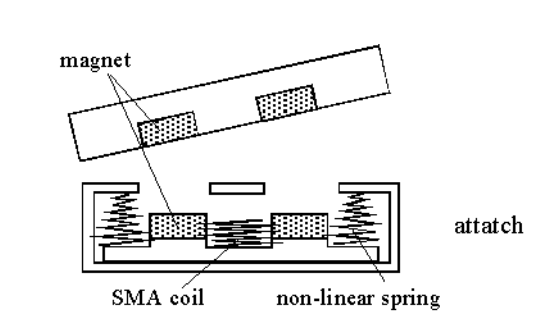
\includegraphics[width=\textwidth]{chapters/res/magnetic_mechanism.PNG}
	\caption{The magnetic docking mechanism described in \cite{murata_hardware_2000}.}
	\label{fig:magnetic_mechanism}
\end{figure}


\section{Assembly protocols}
\label{sec:protocol}
In the context of swarm robotics and this paper, the term assembly protocol is defined as the sequence of actions that has to be performed before a successful self-assembly can occur. 
For pre-programmed robots the protocols is determined by the programmer, and known in advance.
Evolutionary robotics are different in this regard since the controllers are evolved, therefore, the resulting assembly protocols may be unexpected. 
An overview of assembly protocols used in previous projects is presented in table \ref{tab:protocols}.
As for a specific model of an assembly protocol, we have two main approaches. 

\begin{table}[H]
	\centering
	\begin{tabular}{ | l | c | c | c | p{5cm} |}
		\hline
		& Pre-determined & Evolved & Reference\\ \hline
		CONRO & X & & \cite{castano_conro:_2000}\\ \hline
		Miche & X & & \cite{gilpin_miche:_2008}\\ \hline
		SWARM-BOTS project & X & X & \cite{gross_object_2006}\cite{trianni_evolving_2004}\\ \hline
		N/A & & X & \cite{weel_emergence_2012}\\ \hline
	\end{tabular}
	\caption{An overview comparing past research projects of swarm robots based on the robot controller being evolved using an evolutionary algorithm, or pre-programmed for its intended usage.}
	
	\label{tab:protocols}
\end{table}

\subsection{Pre-determined assembly protocol}
The traditional approach is to use an assembly protocol which is determined by the programmer in advance.
This means that the assembly protocol is embedded in the controller software and does not change without reprogramming. 

An example of a pre-determined protocol is found in \cite{gross_object_2006}.
In this experiment, the s-bots uses RGB LEDs to signal their position, and if other s-bots should dock with them.
The lights are also used to determine if the self-assembly process is complete. 

Using the protocol described, the s-bots are successfully self-assembled in 26 out of 30 trials. The advantage of using a pre-programmed assembly protocol is that it can be tailored to the problem. This often leads to good performance and a predictable outcome of the assembly once the system is deployed. It does however carry the disadvantage of being less general in the sense that the protocol can only be changed by implementing new software. Depending on the assembly protocol, it can also be quite complex which in turn, makes the implementation more difficult.

\subsection{Learned assembly protocol}
In a machine learning setting, we can give the robots docking mechanisms, but leave the entire assembly protocol up to the learned controller.
One might ask why machine learning, where the resulting controller rarely is optimal, is a good approach when pre-determined protocols can be developed instead.
According to \cite{russell_artificial_1995}, there are three main reasons for why we would want a robot to learn.
First, the programmer may not always have the ability to foresee all the situations the robot may encounter.
The robot must then learn from its observations if it is to solve the probable new set of problems.
Second, the programmer cannot predict all changes that happen over time. 
If we had some system that tried to anticipate tomorrow's weather, then it must be capable of analysing based on new sets of observation which were unknown at the time of system's design.
And finally, the programmer may not even know the solution to the problem themselves, such that the system itself must find the solution.
This last reason is especially interesting in accordance with self-assembly as we do not always know when it is appropriate to employ self-assembly for solving a certain problem.

An example of a type of learned assembly protocol is found in \cite{trianni_evolving_2004}. 
This example uses s-bots each of which uses an \emph{artificial neural network} to control them. 
The neural network controls all of the input and output signals of the s-bot.
This also includes the use of the gripper(docking mechanism) and the loudspeaker(produces sounds that can be used for communication between the robots).
Using a simple genetic algorithm, they were able to evolve an assembly protocol in 2 out of 10 trials.

Even though an assembly protocol was evolved, the desired results of using the loudspeaker to signal position and performing self-assembly were inconclusive.
The s-bots rather used exploits such as lining up against the wall of the experiment to perform a simpler self-assembly.
The results also showed that the loudspeaker was not used optimally and was something they would like to explore in future research.
This behaviour is one of the disadvantages of using machine learning to develop assembly protocols.
First of all, it may not be able to create a protocol at all, and it is also likely that the end results are sub optimal. 
A reason behind this is that the environment in which the robots are evolved often impacts the type of assembly protocol that emerges.

\section{Machine learning algorithms}
\label{sec:learning}
We say that a robot is learning if it can improve its performance on tasks in the future based on past observations.
Learning ranges from trivial matters such as writing a word to complex theories of the universe.

The learning algorithms commonly used for automatic design of controllers can be divided into two main sub domains: reinforcement learning(RL) and evolutionary algorithms\cite{brambilla_swarm_2013}.

Reinforcement learning is a class of learning algorithms where the agent learns through trial and error, receiving positive and negative feedback for its actions\cite{brambilla_swarm_2013}.
The agent records the feedback received for performing a particular action in each state.
Through this process the agent discovers which action is optimal for a given state.
Applying this form of learning to swarm robotics presents several challenges.
One challenge is the fact that a swarm performs actions as a collective, but the learning is done on an individual level and does not reward global behaviour\cite{brambilla_swarm_2013}.
Additionally traditional RL requires that the environment can be quantized into a finite number of discrete states\cite{schmidhuber_evolutionary_2000}\cite{brambilla_swarm_2013}.
The number of possible interactions between the robots and the environment, and the noise in the real world leads to a high amount of states and makes it difficult to know how these are connected in advance\cite{schmidhuber_evolutionary_2000}.
Techniques such as using an approximator\cite{brambilla_swarm_2013} to reduce the state space, and more intelligent reward mechanisms\cite{brambilla_swarm_2013}, can be used to reduce the impact of these challenges.
Several projects\cite{li_learning_2004}\cite{balch_behavioral_1998}\cite{mataric_interaction_1994} have successfully applied reinforcement learning in multi-agent systems.
Given the challenges of RL, as the goals and ambition of projects increase, researchers are drawn towards techniques that resemble evolutionary algorithms\cite{schmidhuber_evolutionary_2000}.

Evolutionary algorithms attempts to find solutions to a problem by simulating the mechanisms of Darwinian evolution\cite{trianni_evolving_2004}.
In these algorithms, the possible solutions are encoded into genomes and improved iteratively over multiple generations, where well performing individuals reproduce more and spread their genome.



\subsection{Evolutionary algorithms}
\label{sec:evo_alg}
Evolutionary algorithms is a class of algorithm in the category of \emph{bio-inspired algorithms}\cite{binitha_survey_2012}.
Nature has shown that it is a great optimizer.
When we examine features and phenomenons in nature, it tends to find the optimal strategy.
The strategies employed are often very simple, but has great results.
Bio-inspired algorithms takes inspiration from nature and attempts to mimic the behaviour observed in nature.
These algorithms can be categorized by the natural phenomenons they mimic.
The three main categories are \emph{evolution}, \emph{swarm-based}, and \emph{ecology}\cite{binitha_survey_2012}. 
These algorithms are optimization algorithms and can therefore be used to automate the design of robot controllers.
Specifically in the field of evolutionary robotics, the focus has been to employ evolutionary algorithms in the design of robot controllers.


There are many variants of evolutionary algorithms, the most common can be categorized by when the evolution takes place\cite{eiben_embodied_2010}.
\begin{quote} 
	In \emph{off-line} evolution, the evolutionary development of robot controllers takes place before the robots start their “real” operation period.
	\emph{On-line} evolution is the opposite, in that the evolutionary development of robot controllers takes place during the “real” operation period of the robots(although off-line evolution might precede on-line evolution as an educated initialization procedure)and is an ever-continuing process.\cite{eiben_embodied_2010}
\end{quote} 


\subsubsection*{Off-line}
The details of how off-line evolutionary algorithms are implemented usually vary, however most implementations perform a variation of the same following steps\cite{doncieux_evolutionary_2011}, displayed in figure \ref{fig:offline-ea}. 

The first step of an off-line algorithm is to generate some population.
There are two main procedures that can be used to generate the initial population.	 
One can either generate the genomes for the robots completely random, or by some function that applies bias.
In the biological sense, a genome contains the configuration, or blueprint for an individual.
Before the genome can be used by the robots, this configuration must be translated into a robot controller.
The translation procedure can for example consist of translating the genome into an \emph{artificial neural network}, and uploading it to the robots.
The next step after initialization is the robots acting in the environment.
After a given set of time steps, the genome is evaluated by a fitness function which scores the robots based on their ability to solve the task.	 
At the end of a generation, some of the genomes will be selected for reproduction based on their fitness.	 
The algorithm then proceeds to mate genomes through crossover and applying mutation on the population.	 
The process is repeated on this new set of genomes until the desired fitness is reached, or some processing time threshold is met.
\cite{trianni_evolving_2004}\cite{li_co-evolution_2015} describes examples of how this process can be applied to create controllers for self-assembling robots. 

\begin{figure}[H]
	
	\centering
	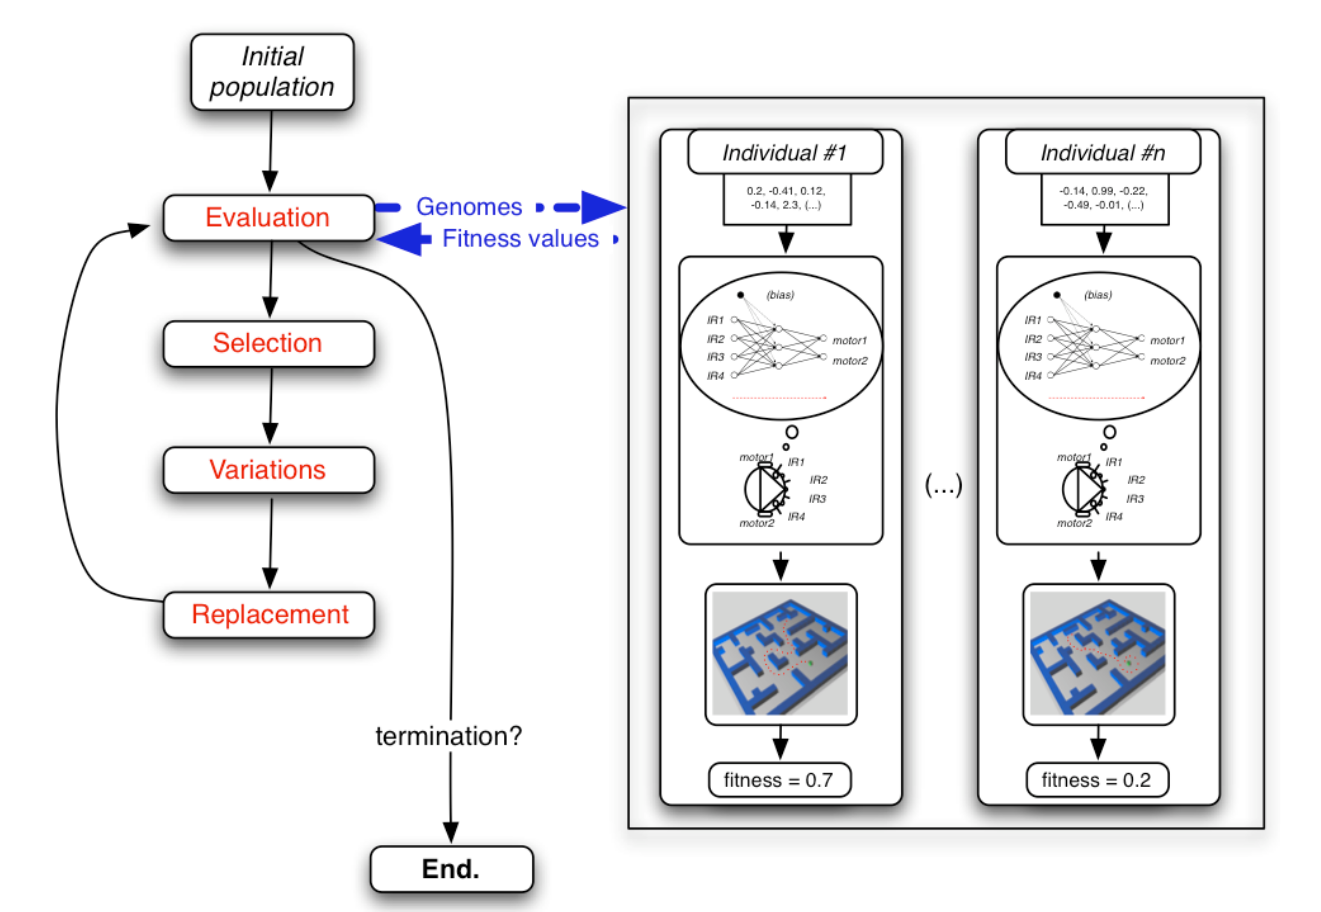
\includegraphics[width=\textwidth]{chapters/res/offline-ea.png}
	\caption{Operation of a typical EA\cite{doncieux_evolutionary_2011}}
	\label{fig:offline-ea}
\end{figure}

The evolution process requires a lot of trials to evaluate the performance of each genome. Performing these trials on real hardware is therefore impractical, time consuming, and possibly dangerous as the robots may damage themselves or the environment.
The evaluation is therefore often performed in simulation\cite{koos_crossing_2010}.
Transferring the controllers evolved in simulation to real hardware has proven to be problematic because the controllers tend to be less efficient once transferred.
This \emph{reality gap} remains a critical issue in evolutionary robotics\cite{koos_crossing_2010}.



\subsubsection*{On-line}
On-line evolutionary algorithms, in contrast to the off-line variants, does not share a well defined series of steps. Several algorithms for this category has been proposed. Among them are mEDEA\cite{montanier_adaptive_2014}, MONEE\cite{noskov_monee:_2013}, and ASiCo\cite{hutchison_task-driven_2011}. 

In mEDEA(minimal Environment driven Distributed Evolutionary Adaptation) each robot contains an active genome and a reservoir of received genomes.
The robots broadcasts their genome in a limited range to other robots.
At a pre-defined number of time steps, the robot forgets its active genome and selects a new one at random from the reservoir.
The robot becomes inactive if it runs out of genomes.
An inactive robot remains stationary for the following generation and receives genomes broadcasted from other robots.
The result is that over time, ineffective genomes are removed from the population while the more successful genomes are able to spread.

MONEE(Multi-Objective and Open-Ended Evolution) can be considered an adaptation of mEDEA.
In MONEE the robot has a life cycle consisting of two phases with a fixed duration.
The first phase is the \emph{life phase}.
In the \emph{life phase}, the robot performs tasks such moving or foraging.
When the lifetime of the robot is reached, it enters a rebirth phase and becomes an "egg".
The egg is stationary and receives genomes from other robots that are currently in their \emph{life phase}.
For the egg to select one genome out of the ones received from the other robots, MONEE introduces the concept of \emph{parental investment}.
During the \emph{life phase} the robots receive credits for performing tasks in the environment.
When a robot passes its genome to an egg, it passes the number of credits earned.
The egg then uses the number of credits to compare and select a new genome for rebirth.
If there are multiple tasks defined, the egg uses an exchange rate between the tasks based on their difficulty to compare them. 
This ensures that genomes who specialize in difficult tasks can compete with genomes that perform easier tasks. 
This system allows genomes to specialize in different tasks and therefore makes MONEE well suited for multi-objective tasks.

ASiCo(Asynchronous Situated Co-evolution) is a co-evolutionary bio-inspired algorithm that in contrast to MONEE and mEDEA uses a fitness function to decide if a robot should reproduce.
Like other on-line algorithms, multiple genomes are present among the robots even though this algorithm carries the characteristic of a fitness function from off-line algorithms.
The ASiCo algorithm works by having the robots act out some scenario and uses energy gain or loss as a performance gauge. 
Differing from off-line algorithms, ASiCo continuously evaluates the different robots' fitness asynchronously.
If a death condition is met, then the robots is either removed from the system or substituted. 
If however a situated mating condition is met, then the candidate is evaluated by its fitness.
If the candidate is acceptable, then it is allowed to reproduce.
In the case where the fitness is not acceptable, it simply continues to live on in the system.

\section{Artificial neural networks}
Computers excel at performing tasks that can be described as a series well-defined steps, and can at these tasks easily outperform humans in doing so.
Tasks that humans find easy, such as understating speech or recognizing faces has proven to be difficult to describe a series of unambiguous operations in the conventional computation model.
Biological neural networks, such as brains, have evolved to be very good at pattern recognition and data classification.
Artificial neural networks(ANN) take inspiration from how biological neural networks process data.

ANN's consist of interconnected processing units(neurons) which work in parallel to solve a specific problem.
The neurons employ a simplified model of how a biological neuron works.
The operation of an artificial neuron consists of two main components, depicted in figure \ref{fig:artificial-neuron}.

\begin{figure}[H]
	
	\centering
	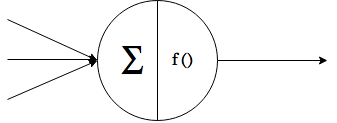
\includegraphics[width=0.5\textwidth]{chapters/res/Neuron.png}
	\caption{Model of an artificial neuron.}
	\label{fig:artificial-neuron}
\end{figure}
First, the neuron sums the action potential from the preceding neurons.
The activation function is then applied on the sum which produces a new action potential as the output.
The role of the activation function is to transform the action potential in the node to an output that can be passed to the succeeding nodes.
These functions often have a thresholding effect where the neuron outputs a low potential until a threshold is reached.
A common activation function is the logistics equation(\ref{eq:logistics-equation}).

\begin{captioneq}[H]
	\begin{equation}
	o_i= \frac{1}{(1+e^{-v})}
	\label{eq:logistics-equation}
	\end{equation}
	
	\caption{The ouput of node i with internal action potential v.}
\end{captioneq}

The connection strength between neurons is simulated by introducing weights on the connections.
A neuron with a higher weight on one of its connections will then be more influenced by that particular connection.
Learning can then be performed by modifying the weights on the connections in the ANN.


The neurons in ANN's are organized into multiple layers, where each neuron is connected to the neurons in the preceding layers.
Typically there is a input layer, an output layer, and zero or more hidden layers between them.

\begin{figure}[H]
	\centering
	\includegraphics[width=0.8\textwidth]{chapters/res/Simple-MLP.png}
	\caption{A feed forward network.}
	\label{fig:mlp-simple}
\end{figure}

Figure \ref{fig:mlp-simple} depicts a simple feed forward network with one hidden layer.
The inputs are propagated from the input layer on the left to the output layer.
More complex network topologies introduce connections within the layers and connections back to preceding layers.

Creating good robot controllers can be difficult as the number of sensors and actuators grow.
The designers may know what desired behavior for the robots is, but expressing this in the conventional computing model as a series of instructions can be difficult.
Instead, with machine learning an ANN can learn from examples of desired behavior provided by the controller designers.
This approach allows designers to create the desired controllers by providing examples instead of knowing the exact solution.

Neural networks have been applied to design robot controllers in several\cite{trianni_evolving_2004}\cite{montanier_adaptive_2014}\cite{brandt_atron_2007} self-assembling robot systems.
These robot systems all use different approaches in how neural networks are applied to create the controller.
\cite{montanier_adaptive_2014} uses a simple feed forward network, while \cite{trianni_evolving_2004} uses a CTRNN, and finally \cite{brandt_atron_2007} uses multiple neural networks which decide different parts of the behavior.
This shows that neural networks are a versatile tool in designing robot controllers for self-assembling robot systems.

